% !TEX TS-program = pdflatex
% !TEX encoding = UTF-8 Unicode

\documentclass[11pt,a4paper,oneside]{book} % use larger type; default would be 10pt

\usepackage[utf8]{inputenc} % set input encoding (not needed with XeLaTeX)

%%% Examples of Article customizations
% These packages are optional, depending whether you want the features they provide.
% See the LaTeX Companion or other references for full information.

%%% PAGE DIMENSIONS
\usepackage{geometry} % to change the page dimensions
\geometry{a4paper} % or letterpaper (US) or a5paper or....
% \geometry{margin=2in} % for example, change the margins to 2 inches all round
% \geometry{landscape} % set up the page for landscape
%   read geometry.pdf for detailed page layout information

\usepackage{graphicx} % support the \includegraphics command and options

% \usepackage[parfill]{parskip} % Activate to begin paragraphs with an empty line rather than an indent

%%% PACKAGES
\usepackage{booktabs} % for much better looking tables
\usepackage{array} % for better arrays (eg matrices) in maths
\usepackage{paralist} % very flexible & customisable lists (eg. enumerate/itemize, etc.)
\usepackage{verbatim} % adds environment for commenting out blocks of text & for better verbatim
\usepackage{subfig} % make it possible to include more than one captioned figure/table in a single float
% These packages are all incorporated in the memoir class to one degree or another...

%%% HEADERS & FOOTERS
\usepackage{fancyhdr} % This should be set AFTER setting up the page geometry
\pagestyle{fancy} % options: empty , plain , fancy
\renewcommand{\headrulewidth}{0pt} % customise the layout...
\lhead{}\chead{}\rhead{\slshape \leftmark}
\lfoot{}\cfoot{\thepage}\rfoot{}

%%% SECTION TITLE APPEARANCE
\usepackage{sectsty}
\allsectionsfont{\sffamily\mdseries\upshape} % (See the fntguide.pdf for font help)
% (This matches ConTeXt defaults)

%%% ToC (table of contents) APPEARANCE
\usepackage[nottoc,notlof,notlot]{tocbibind} % Put the bibliography in the ToC
\usepackage[titles,subfigure]{tocloft} % Alter the style of the Table of Contents
\renewcommand{\cftsecfont}{\rmfamily\mdseries\upshape}
\renewcommand{\cftsecpagefont}{\rmfamily\mdseries\upshape} % No bold!

\usepackage{hyperref} % om \url te kunnen gebruiken

\renewcommand\bibname{Resources} % Bibliography hernoemen

\usepackage{xspace} % automatisch juiste spaties achter macros

\newcommand{\massexpand}{\textsc{mass expand}\xspace} % macro voor Mass Expand

%%% END Article customizations

%%% The "real" document content comes below...

\title{\huge Design and Development of \textsc{Mass Expand},\\ a Bot for StarCraft: Brood War}
\author{Ben Haanstra and Armon Toubman}
%\date{} % Activate to display a given date or no date (if empty),
         % otherwise the current date is printed 

\begin{document}
\maketitle

\frontmatter

\tableofcontents

\listoffigures

\listoftables

\mainmatter

% Introduction
% !TEX root = report.tex

\chapter{Introduction}

In this report, we describe the design and development of a bot that plays the game StarCraft. A StarCraft bot is a computer program or script that plays a game of StarCraft. Our intention for the bot was to be capable of playing without any cheats, adapting to the state of the game and responding quickly. Although we initially pursued the goal of winning as well, we decided to change the focus on being capable of playing properly.

\section{The Game StarCraft}

StarCraft is a real-time strategy game developed by Blizzard and was shipped in 1998. Its foremost expansion Brood War was released later that same year. In general, when one talks about StarCraft, the expansion is implicitly included. Over the years, the game became quite popular as it introduced various interesting gameplay and multiplayer features that easily allowed for communities to grow.

There are three totally different races to be chosen from; the technologic advanced alien race Protoss with access to psionic weaponry and energy shields, the organic alien race Zerg that thrives on evolution and its great numbers to obliterate enemies, and the humanoid race Terran that focuses on conventional weaponry such as machine guns, tanks and nuclear weapons. Each of these races have their own unique units, structures, and their own unique style on how they should be played. In order to build and train those units, the resources Minerals and Vespene Gas have to be harvested and brought back to the main structure of the player.

The other reason that made StarCraft popular was that it is relatively easy to play online against others. This resulted in communities growing and many contests held, with large money prizes. Eventually, professional StarCraft player became a carreer for some. StarCraft was also one of the games used to pioneer \emph{Esports}, the digital variant of sports. In South Korea they showed matches live on television and developed large fanbases, players becoming celebrities, schools and training houses for teams were organized. With the fairly recent introduction of StarCraft II, however, the original game has decreased in popularity. Nevertheless, the game is still regarded as one of the best games made of all times.

The game also features an artificial intelligence, allowing players to try a \emph{skirmish} against the computer. The AI can play at four different levels, ranging from easy to insane, which was a new development at the time. But the AI itself was a very easily programmed script. It did not adapt to the players decisions, was quite repetitive and was easily misled. Furthermore, it cheats by having full observability over the whole field, while the game itself features a \emph{Fog of War} (areas out of sight range are blacked out). It also cheated by having unlimited resources, allowing it to train units even when being economically impaired.

%\begin{figure}
%\centering
%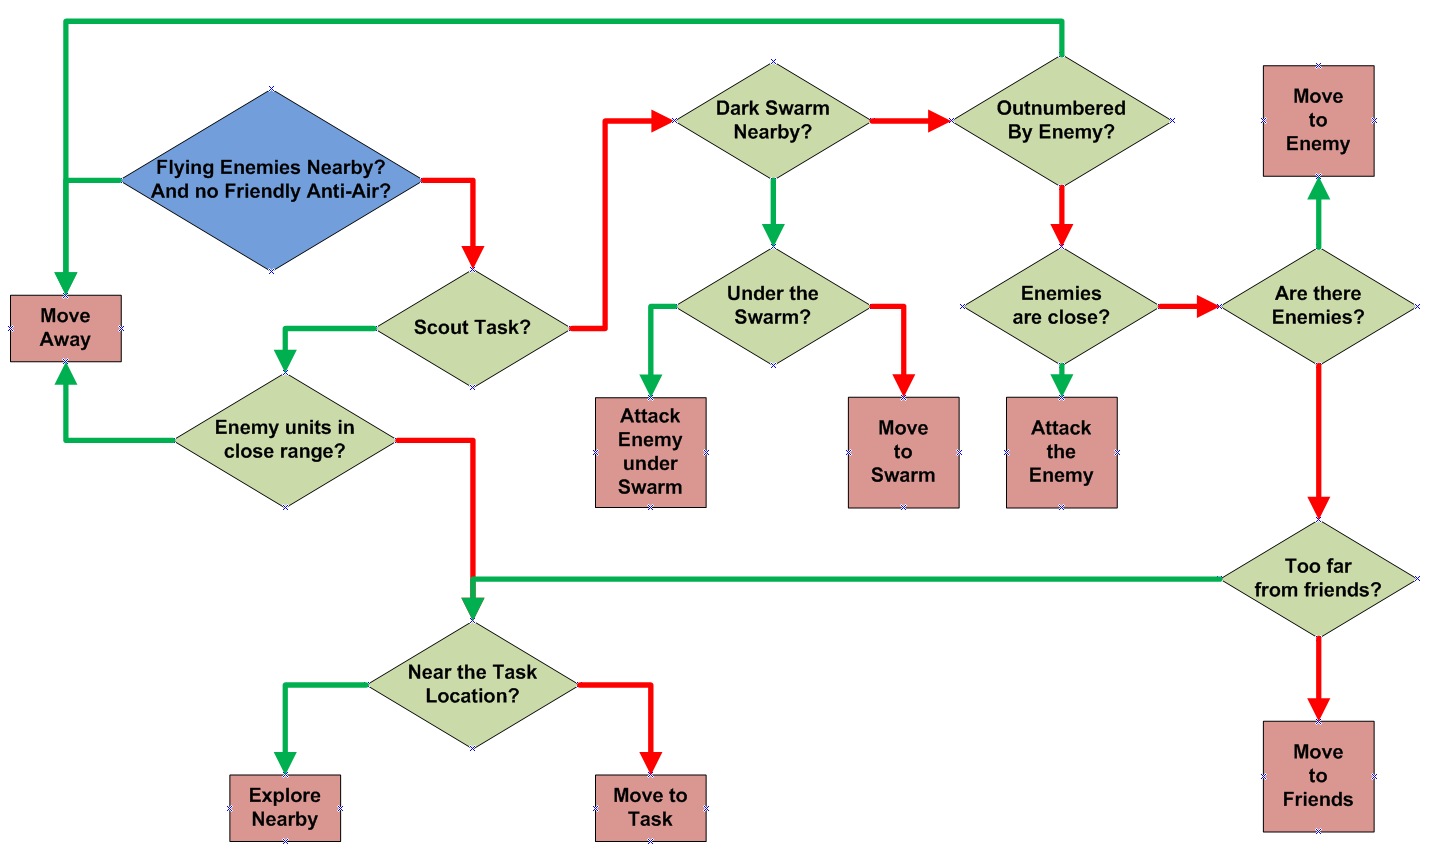
\includegraphics[scale=0.35]{starcraft_zerg_diagram_groot}
%\caption{\label{fig:micro} Flow chart illustration of the decision tree for 'Zergling' units. The blue rhombus is the start and is a decision node. Green rhombi are also decision nodes. Red squares are decision terminals that are to be executed. Green lines indicate a 'yes' answer to the respective question, and red lines indicate 'no'.}
%\end{figure}

\begin{figure}
        \begin{subfigure}[b]{0.5\textwidth}
                \centering
                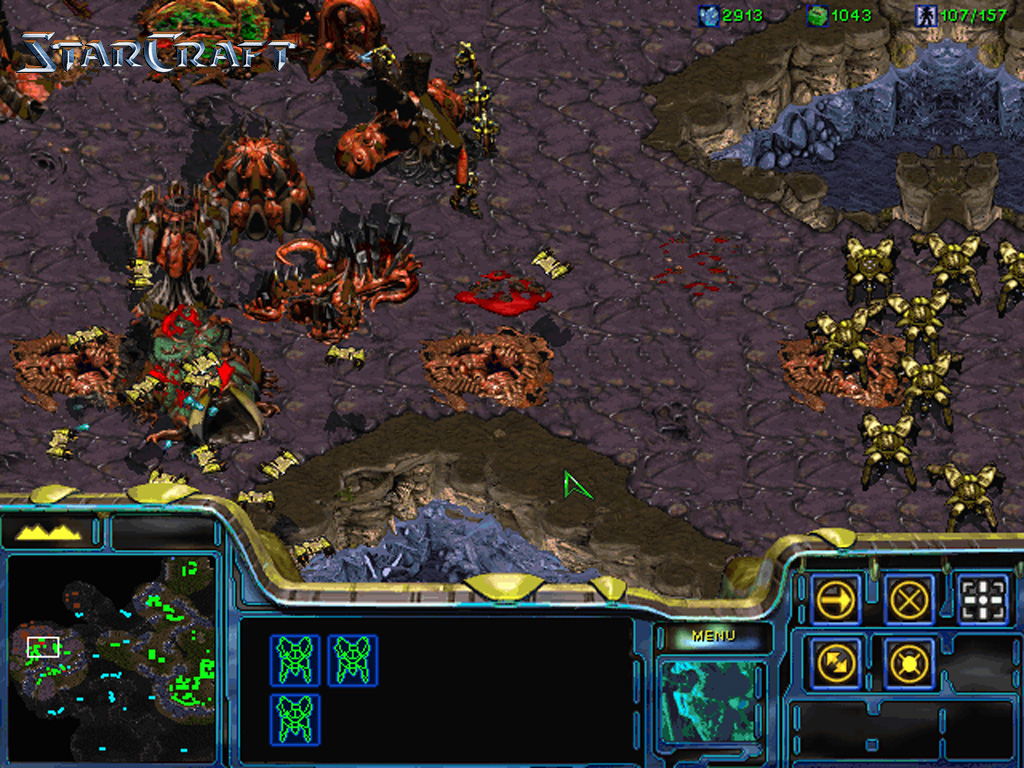
\includegraphics[width=\textwidth]{sc1}
        \end{subfigure}%
        ~ %add desired spacing between images, e. g. ~, \quad, \qquad etc. 
          %(or a blank line to force the subfigure onto a new line)
        \begin{subfigure}[b]{0.5\textwidth}
                \centering
                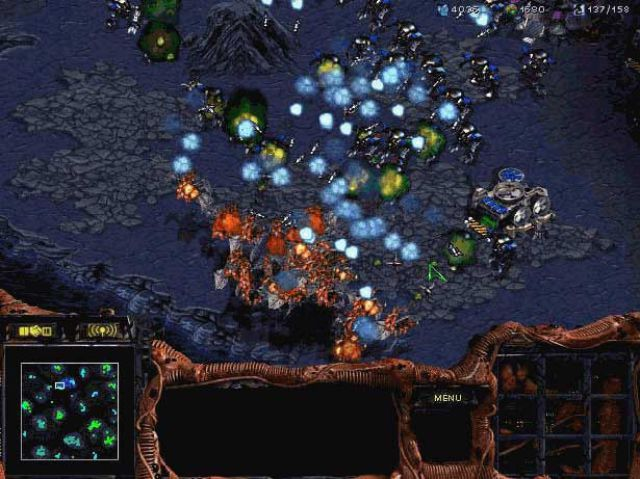
\includegraphics[width=\textwidth]{sc2}
        \end{subfigure}
        ~ %add desired spacing between images, e. g. ~, \quad, \qquad etc. 
          %(or a blank line to force the subfigure onto a new line)
        \caption{Images of battles in StarCraft Brood War}\label{fig:animals}
\end{figure}


\section{Goal of the Bot}
Our goal for the bot is to develop an AI that does not cheat and actually plays the game as it should. To make it more interesting than the standard AI already present in the game, we wanted something that could actually adapt to the playstyle of the opponent and also make its own strategies.

We arrived at this idea for a project when we stumbled upon an announcement for an AI competition for StarCraft, AIIDE2010, meant for bots to play each other. There were four different tournaments one could participate in, from very small scale battle to the complete game. The first two focused on team versus team battles. The third one is a simplified game of StarCraft, where both bots play Protoss, have only access to the units of the lowest tier of technology, and have to gather resources to produce units. The focus of this game is on a more strategic level, as units can not run quickly to the other side of the map. As for the fourth, we have a normal complete game of StarCraft. Although people were free to pick any race, it was adviced to program code for only one specific race. This is because StarCraft is a very detailed game and each race requires a complete different style.

Initially, we started out with the idea to win the competition, but quickly found out that there is a lot more to it than writing just code. Many teams of various universities signed up, some of them having more than 10 members. StarCraft is one of the most complex real-time strategies out there, and developing a very good bot involves a lot of knowledge of the game. Most of this knowledge is unfortunately unwritten and has to be accumulated by playing a lot of times. Knowledge on the top level, however, is prevalently available. For instance, what structures one should build to \emph{counter} the opponent's strategy, or what type of units are good against other type of units. In chapter \ref{chap:strategy}, we go into more detail on how we gathered knowledge.

As a result, we do not aspire to claim our bot is the best, but at least hope to make a versatile bot that can adapt and also initiate combat, without cheating. Furthermore, we wanted to participate in the AIIDE2010 competition's full game tournament, to see how well it works against other bots. As we neared completion of our bot, we decided to name it \massexpand{} referring to its tendency to create many additional bases.


\section{Outline of Report}
We first mention in chapter \ref{chap:libraries} the code made available and details of the competition. In chapter \ref{chap:strategy}, we describe our bot's structure abstractally; AI techniques considered, how units should behave, what overall decisions it has to make, and how we intent to achieve an autonomously adapative bot. The chapter \ref{chap:implementation} then goes into detail on how we implement our bot's strategy. Chapter \ref{chap:timeline} exhibits our timeline of the project and interesting events. We conclude this chapter in \ref{chap:conclusion}, where we also reflect on our choices.


%Many teams signed up, but at the submission deadline only about 30 teams were ready to participate. 





%We started out our project after we came across an Artificial Intelligence (AI) competition for the game; AI2010, a competition meant for bots playing against each other. In this competition, there were four tournaments one could participate in, each tournament having different rules or focus. The first two were focussed on how to control small groups of units, i.e. tactics on how units should work together locally.
%
%The third was a simplified game of StarCraft, were only units and structures of the lowest tier of technology were available. Here, the focus shifts more to placing units appropriately over the map. 
%%% We participate in the AI2010 competition

% Project goals (project voor vak, meedoen aan toernooi)

% Programming tools (bwapi/bwsal/bwta)

% Architecture (schema van geheel, beschrijving van alle onderdelen)
% !TEX root = report.tex

\chapter{Bot Architecture}
\label{chap:implementation}

This chapter will describe the overall structure of \massexpand and provide descriptions of the major components.

\section{Overall Structure}

The starting point of the creation of the bot was the example AI module distributed with BWAPI. The example contains the main update loop of the bot, all event listeners BWAPI supports and methods for drawing extra information on the screen. It also provides some sample code for giving orders to units. We left the example module mostly intact, except for the units orders which we removed completely. We added calls to methods of a new class, HighCommand, which would be the control center for our code. The main benefits of this were that we kept the example code for reference, and that if there would be a major change in BWAPI, we could use the new example module and quickly plug in our own code.

In our first attempts to create a bot, we tried using BWSAL, a collection of classes forming an abstraction layer for BWAPI. These classes provide methods for common tasks such as assigning workers to collect resources, maintaining a build queue and finding suitable building places. We quickly abandoned BWSAL after realizing it would be hard to adapt it to our ideas. What we kept from BWSAL were two helper classes, UnitGroup (an excellent class to select and divide groups of units) and BuildingPlacer (a class with methods to determine where a building should be built). We also kept the overall structure BWSAL used, including the naming scheme (the "managers").

The managers are all responsible for a part of the performance of the bot. For example, we have a manager keeping track of our minerals and gas, a manager storing information about enemy units and a manager overseeing construction of buildings and units. Organizing the bot this way allows us to seperate code pertaining to different areas of the bot operation, and also allows us to structure the way the information obtained from the game flows through our bot, resulting in commands sent back to the game. This flow of information is shown in Figure~\ref{fig:flowofinformation}.

\begin{figure}[htb]
\centering
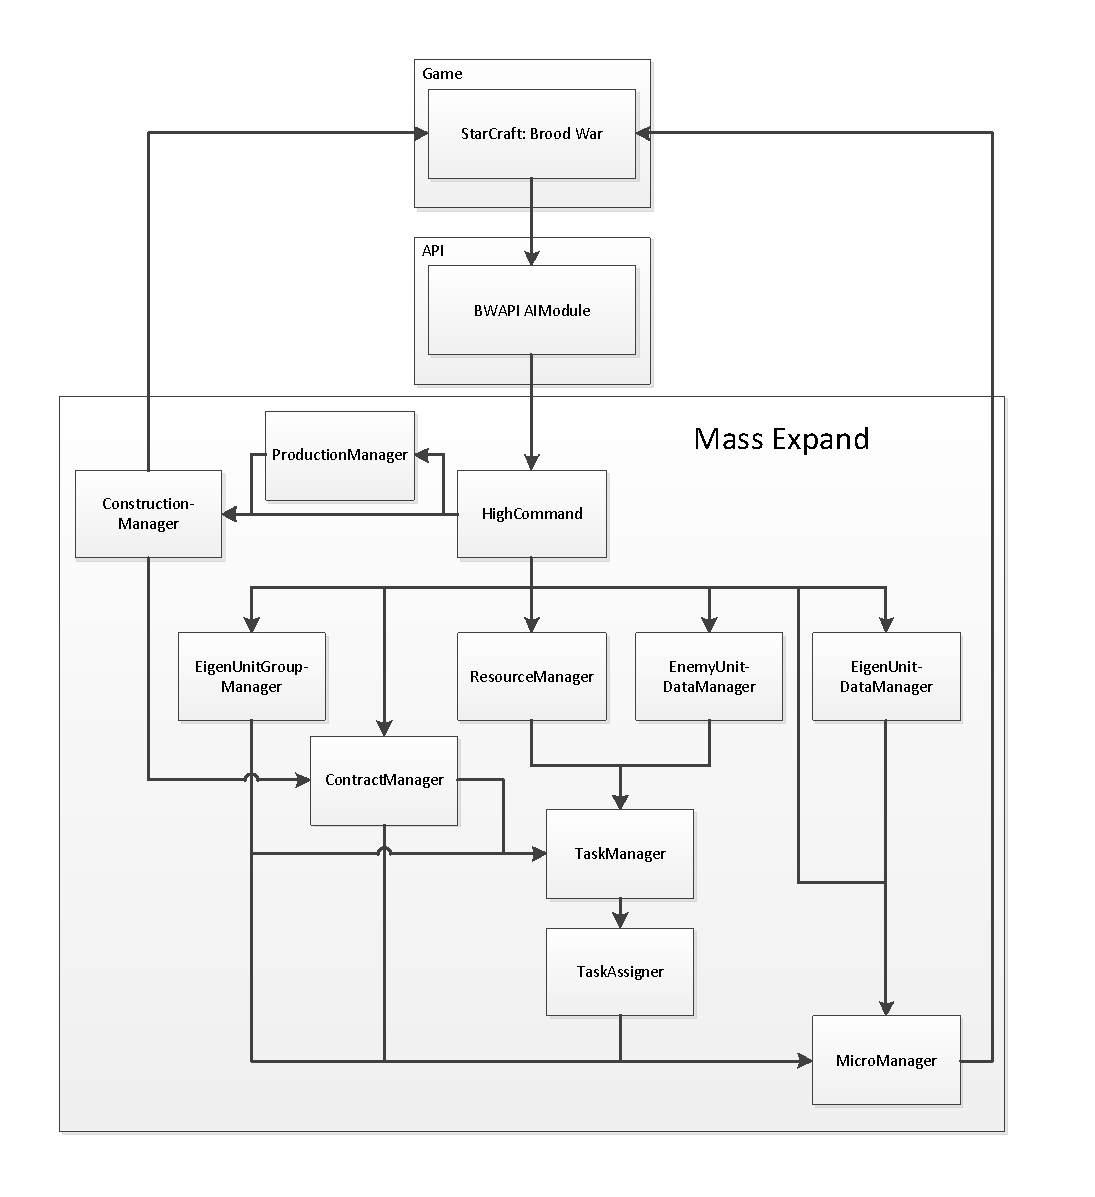
\includegraphics[width=\textwidth, trim= 0mm 30mm 0mm 30mm, clip]{images/flowofinformation}
\caption{The flow of information from StarCraft through Mass Expand to MicroManager and ConstructionManager, which send commands back to StarCraft.}
\label{fig:flowofinformation}
\end{figure}

Figure~\ref{fig:flowofinformation} can also be seen as a parallelized version of the main loop of our bot. However, in practice, the managers are called in serial form. When the update function of HighCommand is called (which is our main loop), it tells the managers to update in the following order:

\begin{description}
\item[EigenUnitDataManager] Data about our own units is updated.
\item[EigenUnitGroupManager] Any new units we have are assigned to persisting unitgroups, small groups are merged and large groups are split up.
\item[ResourceManager] Lists of mineable gas and mineral deposits close to our bases are updated.
\item[EnemyUnitDataManager] Data about visible enemy units is updated, such as their position and health.
\item[ProductionManager] Plans are made for the construction of buildings, units, upgrades and technology.
\item[ConstructionManager] Plans made by ProductionManager are executed if possible.
\item[ContractManager] Build orders for buildings are delegated to drones and a suitable build location is found for them.
\item[TaskManager] Tasks are collected from the other managers.
\item[TaskAssigner] The collected tasks are assigned to units and unitgroups.
\item[MicroManager] Mobile units are given specific movement instructions, based on their tasks and enemies near their location.
\end{description}

HighCommand and the managers will be described in more detail in the following sections.

\section{HighCommand}

HighCommand is the control center of our bot. It does three things:

\begin{itemize}
\item It instantiates the managers and calls them in the right order.
\item It listens for game events from BWAPI and forwards them to the right managers.
\item It draws extra textual and graphical information on top of the game interface.
\end{itemize}

The specific order in which HighCommand calls the managers is listed in the previous section. The order is important because some managers require updated information from other managers to function.

BWAPI allows AI modules to draw extra information on the screen, on top of the game interface. This is a handy feature to show internal information of the bot that would otherwise be invisble. HighCommand currently calls these functions to display the location and type of tasks, the assignment of units to tasks (shown as lines from units to tasks), the build queue and current contracts (drones that are ordered to build a structure).

\section{EigenUnitDataManager}

EigenUnitDataManager records data about our own units (\emph{eigen} means own in Dutch). BWAPI provides many methods to get data about our own units, but this data might change each frame. By recording data from the last frame, we are able to detect changes. One of such changes we monitored was a loss of hit points, which indicated a unit was being attacked (BWAPI later added a function to detect whether a unit was under attack). Another option this manager provides is to record which of our units were seen by the enemy and where and when this occured. If one of our units ever moved within visual range of an enemy unit, we can be sure the enemy knows about that unit and will act on that information. On the other side, we can use unseen units to our advantage (such as using them for a surprise attack).

\section{EigenUnitGroupManager}

This manager divides all our mobile units into persistent groups. Such groups can be manipulated as if it were a single unit: orders given to a unitgroup are passed to all the units in the group. Unitgroups are implemented in the UnitGroup class from BWSAL, which provides many helpful selector functions, such as "get all flying units in this group". The selector functions can be chained, allowing us to manage our units with very concise code.

The groups that the EigenUnitGroupManager maintains are updated whenever the number of units we have is changed. When a new unit is created, it is either assigned to an existing group or given its own new group. When one of our units dies or we otherwise lose control of it, it is removed from its group. The groups are then balanced by reassigning units between groups, according to various rules.

For example, new Overlords are always given a new group of their own. However, if there is a group of Mutalisks that does not have any Overlords, the Overlord will be moved to the Mutalisk group in the balancing step. It is handy to have a Overlord with Mutalisks (both flying units) because the Overlord can detect stealth units, which are then easily taken out by the Mutalisks.

Drones are a special case. We keep all Drones in a single group. While they are capable of combat, they are mostly used for gathering resources and construction. By keeping them in a special group we make sure they are not accidentally assigned to combat tasks. The drone group has a constant pointer, allowing easy access to all drones.

\section{EnemyUnitDataManager}

EnemyUnitDataManager keeps track of enemy units. By default, BWAPI only allows access to visible units. However, we we want to retain information about them when they become inaccessible, such as when they use a stealth ability or move into fog of war. Units can also transform into a different unittype. In that case, we need to make sure we recognize it as the same unit instead of counting it as two seperate units. The manager currently records five pieces of information about each enemy unit we encounter: its type, its hitpoints, its position, its last known position, and the time at which it was last seen by us. This information is saved together with a pointer to the unit.

There is an important difference between the position and the last known position. While an enemy unit is visible, we update its position, and its last known position is changed to that position. When it moves somewhere we cannot see it (for example, into fog of war) we change its position to "unknown" and keep its last known position. We can then send scouts to make that position visible. If the unit is still there, we can update its position again.

The information kept by this manager is used to create combat and scout tasks, but could also for example be used to determine the technological progress of the enemy and make predictions about the tactics the enemy will use.

\section{ResourceManager}

There are two main resources in StarCraft that have to be gathered: gas and minerals. Without these, you cannot build buildings and units, purchase upgrades and research technology. Minerals are mined from mineral patches by workers. Gas is gathered from extractors that have to be built atop geysers. Once gathered, the resources are dropped off by the workers at resource deposits. For the Zerg, the resource deposit is a Hatchery or one of its upgraded forms (Hive or Lair). Mineral patches and geysers are usually grouped together at certain locations on the map, called base locations. It makes sense to establish bases at these locations, to gain control of and allow easy gathering of the resources.

The ResourceManager catalogs the resources available at our bases. It keeps track of mineral patches, geysers and gas extractors near our bases. Since geysers are ungatherable without an extractor, it notifies the managers concerned with building when we have available geysers. The manager also creates tasks for our mineral patches and gas extractors, so that drones can be assigned to gather resources from them.

This manager needs to be kept updated for a number of reasons. Mineral patches and geysers can be exhausted after which they will no longer provide resources. Second, gas extractors are buildings and can be destroyed. Also, when new bases (expansions) are created, new resources on that location usually become available. The way this manager decides which resources are "ours" (by checking their distance to our bases) also prevents the bot from sending workers to resources being mined by the enemy, most likely resulting in the death of our workers.

\section{TaskManager}

Some of the managers (currently EnemyUnitDataManager and ResourceManager) create tasks based on their data. The job of the TaskManager is to collect these tasks, group them into categories and prepare them for assignment. Tasks have information associated with them such as a location and a target unit. The categories are:

\begin{description}
\item[ScoutTask] Created for locations we want visible.
\item[CombatTask] Created for each visible enemy unit.
\item[PrepareTask] This task is for gathering armies, so they don't go attack in small groups which is ineffective.
\item[DetectorTask] When an enemy unit uses a stealth ability, we create want an Overlord to try and expose it at its last known location.
\item[DefendTask] Created for locations that we want to defend with extra military units.
\item[GatherMineralsTask] Created for minerals we want workers to gather.
\item[GatherGasTask] Created for gas we want workers to gather from extractors.
\end{description}

The TaskManager also creates some tasks itself. In the beginning of the game, it creates ScoutTasks for each base location. This results in Overlords flying across the map to find the enemy's starting location. Later in the game, when we have reached a certain number of units, we want all base locations visible at all times, to expose any expansions the enemy might have created.

\section{TaskAssigner}

The tasks collected by the TaskManager are taken by the TaskAssigner to assign them to unit groups. For each group, the TaskAssigner goes through all the collected tasks and compiles three lists: ideal tasks, good tasks and bad tasks. Tasks that are best fitted to the group are put in the ideal tasks list. Tasks that could be done by the group but are best left for another group are put into the good tasks list. Bad tasks are tasks that should not be done by this group, or may even be impossible to be performed by the group. The group is then assigned an ideal task. If there is none, it is assigned a good task. If there is no good task either, it is assigned a bad task.

What constitutes an ideal, good or bad task for a group is determined by a set of rules. For example, DetectorTasks are ideal tasks for Overlords and not even considered for other groups with other units because Overlords are the only units that can detect stealth units. ScoutTasks are always good tasks for Overlord. By not making ScoutTasks ideal for Overlords, we ensure that DetectorTasks take priority during assignment. CombatTasks are bad for Overlords because they have no combat abilities.

Since TaskAssigner assigns tasks to unit groups, and EigenUnitGroupManager seperates Drones from the other units, Drones are also assigned tasks seperately. Currently they are only assigned gathering tasks. They are also capable of doing ScoutTasks and CombatTasks but that is not implemented in the current decision rules.

\section{ProductionManager}

The ProductionManager decides two things: which buildings, technology and upgrades (henceforth called tech) we should have, and what tech are going to build right now. These decisions are kept in what we call the wantlist and the buildlist.

We identify a number of stages in terms of at what tech we should have. Each of these stages is defined by a set of tech. When we have all the desired tech, we move up one stage. The tech defined by the current stage is kept in the wantlist. Simply put, we want the tech that is in the wantlist.

When the ProductionManager sees tech in the wantlist that we have not actually built yet, it copies that tech into the buildlist. The buildlist can be seen as an ingame build queue. The manager also adds units to the buildlist. The type of units we want to build is determined according to a set of rules. These rules take into account information such as at what stage we are (and thus what units we can actually build), enemy units that we have seen, and the race of the enemy. The list of rules is extensive, and can be said to form the heart of the strategy of \massexpand .

\section{ConstructionManager}

The ConstructionManager takes the buildlist from the ProductionManager and tries to realize as much of the tech as possible. The only limiting factor is our resources.

If we can afford the first item in the list in terms of gas, minerals and supply, and we have the technological capability of building or researching the item, the order to purchase it is sent to the appropriate unit. In case the first item is a building, the ContractManager is told to create a new Contract (more on this later). We then check to see if we can afford the second item, taking into account the resources we just used on the first item. Once we can't afford an item, the process is stopped.

The ConstructionManager and the MicroManager are the only managers that send orders back to StarCraft. When we purchase a unit, an upgrade or a technology, the ConstructionManager looks up which unit builds or researches it with helpful methods from BWAPI and sends the right orders to that unit.

\section{ContractManager}

Orders to to build new buildings are given to Drones by specifying the type of building we want and the location where we want it. The Drone then moves to that location and morphs into the building. However, between giving the order and the Drone reaching the desired location, a lot can happen. The Drone could for example run into enemies and be killed or otherwise stopped from accomplishing its task. This is why we have come up with the ContractManager.

For each building we want built, we tell the ContractManager to create a Contract. Drones are then assigned to Contracts without a contractor. Contracted Drones are given a building location and are told to move there and build the desired building. The Contracts allow us to keep track of which desired buildings have been built. This way, when a Drone is killed en route to its destination, the ContractManager sees that the contracted Drone has died and will assign another Drone to the Contract (and perhaps a different building location). This method also ensures that building orders for specific buildings are given only once. In the past, there have been problems with multiple Drones taking the same orders, leading to an exodus of Drones to a single building spot, all of them blocking each other's building sites. The use of Contracts now prevent this behaviour.

\section{MicroManager}

The MicroManager is what makes \massexpand move. The name comes from micromanagement: detailed management of units in combat. The MicroManager sends orders to move and attack to our mobile units. The specific orders are determined by decision trees.

There is a decision tree for each type of unit. At the beginning of the tree, the task of the unit is retrieved. Decisions are then made based on this task and the unit's surroundings. For example, Drones are usually assigned to gather the resource pointed to in their task, but may be forced to fight in case their base is under attack. Mutalisks are to engage the enemies pointed to by their combat tasks, but have to do so with special maneuvers. Overlords have to reach their scouting tasks, but avoid anti-air defenses. There are too many details to describe here.

The manager usually iterates through all units and runs them through the decision trees. To speed up this process, we have given the manager the ability to grab nearby groups of units and give them the same orders. This is especially handy in combat situations, because enemy units can be brought down fast with focus fire.

% Strategy
%    Micro
%    Bouwen

% Evaluation (testresultaten)

% Conclusion

\backmatter

% Tijdlijn
% !TEX root = report.tex

\chapter{Project Timeline}

\paragraph{January 2010}
Found announcement for the AIIDE 2010 StarCraft Competition. Team \massexpand is born.

\paragraph{February 2010 - June 2010}
The Game Programming course is given at the University of Amsterdam and followed by both team members. A proposal to submit the bot as the final project for the course is accepted.

\paragraph{August 2010 - September 2010}
The first version of \massexpand is ready. The bot plays well but suffers from slowdowns and crashes.

\paragraph{September 2010 - October 2010}
The competition is held at UC Santa Cruz in California, USA. \massexpand participates in tournament 4 (complete games).

\paragraph{November 2010}
The results are posted online. \massexpand won the first round 1-3, but then lost 0-3 to the bot which would continue to win the tournament.

\paragraph{August 2011}
Work continues on a second version. The code is rewritten from scratch and uses the latest version of BWAPI, hoping to eliminate the slowdowns and crashes. This version will be submitted for the Game Programming course.

\paragraph{September 2011}
Finishing work on the bot and the documentation.

% Resources (links naar source/docs/bwapi etc.)
% !TEX root = report.tex

\nocite{*}

\begin{thebibliography}{99}

\bibitem{massexpandproject}
	MassExpand project page.\\
	\url{http://code.google.com/p/massexpand/}

\bibitem{massexpanddocs}
	MassExpand code documentation.\\
	\url{http://www.armontoubman.com/massexpand/html/index.html}

\bibitem{starcraft}
	Blizzard Entertainment: StarCraft.\\
	\url{http://us.blizzard.com/en-us/games/sc/}

\bibitem{aiidecomp}
	AIIDE 2010 StarCraft AI Competition page.\\
	\url{http://eis.ucsc.edu/StarCraftAICompetition}

\bibitem{bwapi}
	BWAPI project page.\\
	\url{http://code.google.com/p/bwapi/}

\bibitem{bwsal}
	BWSAL project page.\\
	\url{http://code.google.com/p/bwsal/}

\bibitem{bwta}
	BWTA project page.\\
	\url{http://code.google.com/p/bwta/}

\bibitem{liquipedia}
	Liquipedia StarCraft Strategies \\
	\url{http://wiki.teamliquid.net/starcraft/Main_Page}

\bibitem{videos}
	Replay videos for knowledge elicitation: consulted YouTube channels and archives \\
	\url{http://eis.ucsc.edu/StarCraft_Data_Mining}\\
	\url{http://www.gosugamers.net/starcraft/replays/}\\
	\url{http://www.teamliquid.net/replay/}\\
	\url{http://www.youtube.com/user/ESportsTV}\\
	\url{http://www.youtube.com/user/nevake}\\
	\url{http://www.youtube.com/user/Jon747}\\
	\url{http://www.youtube.com/user/StarCraftLegacy}


\end{thebibliography}

\end{document}
